\documentclass{beamer}
\usetheme{Berkeley}
\usecolortheme[RGB={132,184,24}]{structure} 
\usepackage[utf8x]{inputenc}
\usepackage{ucs}
\usepackage{amsmath}
\usepackage{amsfonts}
\usepackage{amssymb}
\usepackage{enumerate}
\usepackage{listings}
\lstdefinelanguage{JavaScript}{
  keywords={typeof, new, true, false, catch, function, return, null, catch, switch, var, if, in, while, do, else, case, break},
  keywordstyle=\color{blue}\bfseries,
  ndkeywords={class, export, boolean, throw, implements, import, this},
  ndkeywordstyle=\color{darkgray}\bfseries,
  identifierstyle=\color{black},
  sensitive=false,
  comment=[l]{//},
  morecomment=[s]{/*}{*/},
  commentstyle=\color{purple}\ttfamily,
  stringstyle=\color{red}\ttfamily,
  morestring=[b]',
  morestring=[b]"
}
%\lstset{
%   language=JavaScript,
%   backgroundcolor=\color{lightgray},
%   extendedchars=true,
%   basicstyle=\footnotesize\ttfamily,
%   showstringspaces=false,
%   showspaces=false,
%   numbers=left,
%   numberstyle=\footnotesize,
%   numbersep=9pt,
%   tabsize=2,
%   breaklines=true,
%   showtabs=false,
%   captionpos=b
%}

\logo{\pgfimage[width=15.7mm]{tudo127x97.jpg}}
\title{JavaScript und DOM-Scripting}
\begin{document}
\frame{
	\frametitle{Thema: JavaScript und DOM-Scripting}
	\tableofcontents
	[pausesections]
}
\section{Aufgabe 2.1: Clientseitige Formularvalidierung}
\begin{frame}{Aufgabe 2.1}
\begin{center}
Implementierung einer clientseitigen Formularvalidierung mithilfe von JavaScript (innerhalb der HTML-Datei):\\
~\\~\\
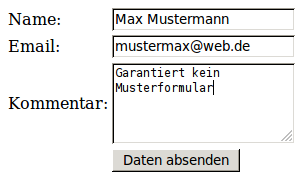
\includegraphics[width = 120px]{../A1/src/formvali.png}
\\
Betrachtet werden die für die Aufgabe relevanten $\langle${\bf form}$\rangle$ - und $\langle${\bf script}$\rangle$ -Blöcke:
\end{center}
\end{frame}


\tiny{\begin{lstlisting}[language = HTML,
				   mathescape = true, 
                   morekeywords = {onsubmit, onclick, this, return}, 
                   numbers = left, 
                   numbersep = 3pt]
 <form name = "vali" method = "post" action = "aufgabe2_1.html"
 onsubmit = "return$~$validate(this);">
<table border= "0" cellpadding= "0" cellspacing= "4">
 <tr>
  <td align = "left">Name:</td>
  <td align = "left">
  <input type = "text" name = "nameTextField" size = "20"></td>
 </tr>
 <tr>
  <td align = "left">Email:</td>
  <td align = "left">
  <input type = "text" name = "eMailTextField" size = "20"></td>
 </tr>
 <tr>
  <td align = "left">Kommentar:</td>
  <td align = "left">
  <textarea name = "commentTextArea" rows = "4" cols = "15">
  </textarea></td>
 </tr>
 <tr>
  <td align = "left"></td>
  <td align = "left">
  <input type = "button" value = "Daten$~$absenden" name = "validateButton" 
   onclick = "validate(this);"></td>
 </tr>
</table>
</form>
\end{lstlisting}}

\begin{frame}{Anmerkungen zum $\langle$form$\rangle$ - Block}
\normalsize{
\begin{itemize}
\item Bevor die Daten abgeschickt werden können, muss {\bf onsubmit = $"true"$} sein.
\item Durch einen Klick auf den Button {\bf Daten absenden} überprüft die Methode {\it validate()}, ob alle Angaben korrekt sind (true) oder nicht (false).
\end{itemize}}
\end{frame}

\tiny{
\begin{lstlisting}[language = JavaScript,
				   mathescape = true, 
                   numbers = left, 
                   numbersep = 3pt]
<script type="text/javascript">
function validate() {
  var name        = document.vali.nameTextField.value;
  var eMail       = document.vali.eMailTextField.value;
  var comment     = document.vali.commentTextArea.value;
  var regExpName  = /([a-zA-Z]{2,})\s([a-zA-Z]{2,})/i;
  var regExpMail  = /^(\w[\w.]{2,}@)(\w{2,}.)*([a-zA-Z]{3,}\.[a-zA-Z]{2,4})/$\$$i;
	
  if(name != "" && eMail != "" && comment != "") {
	 if(regExpMail.test("" + eMail) == false) {
		 alert("Ungueltige Emailadresse.");
		 return false;
	 }
	 else if(regExpName.test(name) == false) {
		 alert("Ungueltiger$~$Name.$~$Namen$~$in$~$der$~$Form$~$\n$~$
		 Vorname<Leerzeichen>Nachname$~$angeben.");
	 }	
	 else { 
		 alert("Daten$~$wurden$~$erfolgreich$~$abgeschickt.$~$\n$~$Ihre$~$Daten:$~$\n$~$
		 Name:$~$" + name + "\n$~$Email:$~$" + eMail + "\n$~$Kommentar:$~$" 
		 + comment);	
		 return true;	
	 }
  }
  else {
	 alert("Es$~$wurden$~$noch$~$nicht$~$alle$~$Felder$~$ausgefuellt.");
	 return false;
  }
};
</script>
\end{lstlisting}}

\begin{frame}{Anmerkungen zum $\langle$script$\rangle$ - Block}
\small{
\begin{itemize}
\item {\it validate()} überprüft mittels regulärer Ausdrücke\\ (Zeile 6 u. 7) die Angaben auf Korrektheit:
	\begin{itemize}
	\item {\bf Name} hat die Form Vorname$\langle$Leerzeichen$\rangle$Nachname
	\item {\bf Emailadresse} hat die Form \newline [min. 3 Zeichen ]@[min. 3 Zeichen].[2 - 4 Buchstaben]
	\end{itemize}
\item Bei einer ungültigen Eingabe oder nicht ausgefüllten Feldern erscheint eine Fehlermeldung in Form einer Alert-Box .
\item Sind alle Angaben korrekt, erscheint eine Alert-Box mit den angegebenen Daten.
\end{itemize}}
\end{frame}

\section{Aufgabe 2}
\begin{frame}{Aufgabe 2}
\end{frame}

\section{Aufgabe 2.3: Tooltip-Fenster}
\begin{frame}[<+->]{Aufgabe 2.3}
\normalsize
\begin{itemize}
\item Erstellen einer Tooltipbibliothek.
\item Tooltips bewegen sich mit der Maus.
\item Tooltips erscheinen erst nach einer bestimmten Anzahl an Millisekunden.
\item Die Bibliothek lässt sich ohne großen Aufwand in bestehende HTML-Dokumente einbinden.
\end{itemize}
\end{frame}
\tiny{\begin{lstlisting}[language = HTML,
                                   mathescape = true, 
                   breaklines=true, 
                   numbers = left, 
                   numbersep = 3pt]
<!DOCTYPE HTML PUBLIC "-//W3C//DTD HTML 4.01 Transitional//EN" "http://www.w3.org/TR/html4/loose.dtd">
<html>
    <head>
        <meta http-equiv="Content-Type" content="text/html; charset=utf-8">
        <title>Tooltip Beispiel</title>
        <script type="text/javascript" src="jstooltip.js"> </script>
        <script type="text/javascript">
                addTooltip('name', 'message', 1000);
                addTooltip('email', 'message2', 1000);
        </script>
    </head>
    
    <body>
		<form action="" method="get">
			<fieldset>
            	<legend>Eingaben</legend>
                <label>Name:</label>&nbsp;<input id="name" type="text"><br>
                <label>E-Mail:</label>&nbsp;<input id="email" type="text">
                <input id="abschicken" type="submit" value="Abschicken">
			</fieldset>
		</form>    	
    </body>
</html>
\end{lstlisting}
}
\normalsize
\begin{frame}[<+->][fragile]
\tiny{\begin{lstlisting}[language = HTML,
			numbers=left,
			firstnumber=6,
			numbersep = 3pt]
        <script type="text/javascript" src="jstooltip.js"> </script>
        <script type="text/javascript">
                addTooltip('name', 'message', 1000);
                addTooltip('email', 'message2', 1000);
        </script>
\end{lstlisting}}
\pause
\begin{itemize}
\normalsize
\item Zeile 6 bindet die Bibliothek ein
\item Zeile 8 und 9 zeigen, wie man HTML Elementen einen Tooltip hinzufügt.
\end{itemize}
\end{frame}
\begin{frame}[<+->]
\begin{itemize}
\item Funktionen der Bibliothek
\begin{description}
\small
\item[addTooltip] Wrapperfunktion, die \textbf{addTooltip\_} aufruft, sobald das Dokument geladen hat.
\item[addTooltip\_] Fügt unsichtbar dem Dokument alle Tooltips hinzu und erweitert die Elemente, die einen Tooltip bekommen um \textbf{onmouseover}, \textbf{onmousemove} und \textbf{onmouseout} Events.
\item[showTooltip] Positioniert den Tooltip und startet einen Timer, um ihn sichtbar zu machen.
\item[hideTooltip] Stoppt den Timer und versteckt den Tooltip wieder.
\item[moveTooltip] Positioniert den Tooltip anhand der Maus neu.
\end{description}
\normalsize
\item Globales Array
\small
\begin{description}
\item[timeout]Enthält die laufenden Timer, um bei Verlassen eines Elementes den Tooltiptimer abzubrechen.
\end{description}
\end{itemize}
\end{frame}
\begin{frame}[<+->][fragile]
\tiny{\begin{lstlisting}[language=JavaScript, 
		   numbers=left,
		   numbersep=3pt,
		   breaklines=true]		 
timeout = new Array();

function addTooltip(Id, tooltip, milliseconds) {
        document.addEventListener('DOMContentLoaded', function(e){
                addTooltip_(Id, tooltip, milliseconds);
        }, false);
}
\end{lstlisting}}
\normalsize
\begin{description}
\item[Problem]Man kann nicht auf auf HTML Elemente zugreifen, wenn sie noch nicht geladen sind.
\item[Lösung]Wir warten, bis das Dokument vollständig geparst ist
\end{description}
\end{frame}
\begin{frame}[<+->][fragile]
\tiny{\begin{lstlisting}[language=JavaScript, 
		   numbers=left,
		   numbersep=3pt,
		   breaklines=true,
		   firstnumber=8]
function addTooltip_(Id, tooltip, milliseconds) {
        var element=document.getElementById(Id);
        tooltipId = "tooltip"+Id;
\end{lstlisting}}
\normalsize
\pause
\begin{itemize}
\item Zugriff auf das Element, welches den Tooltip bekommt.
\item Aus der ID wird eine TooltipId generiert.
\end{itemize}
\end{frame}
\begin{frame}[<+->][fragile]
\tiny{\begin{lstlisting}[language=JavaScript, 
		   numbers=left,
		   numbersep=3pt,
		   breaklines=true,
		   firstnumber=11]
        var tooltipdiv = document.createElement("div");
        tooltipdiv.id=tooltipId;
        tooltipdiv.innerHTML=tooltip;
        tooltipdiv.style.position="absolute";
        tooltipdiv.style.backgroundColor="#ffffff";
        tooltipdiv.style.border="1px solid #72B0E6";
        tooltipdiv.style.font="12px Verdana";
        tooltipdiv.style.color="#1A80DB";
        tooltipdiv.style.display="none";
        document.body.appendChild(tooltipdiv);
\end{lstlisting}}
\normalsize
\pause
\begin{itemize}
\item Ein div-Element wird für den Tooltip generiert, versteckt und dem Dokument hinzugefügt.
\end{itemize}
\end{frame}
\begin{frame}[<+->][fragile]
\tiny{\begin{lstlisting}[language=JavaScript, 
		   numbers=left,
		   numbersep=3pt,
		   breaklines=true,
		   firstnumber=21]
        element.setAttribute("onmouseover", "showTooltip(event,'"+tooltipId+"', '"+tooltip+"',"+milliseconds+");");
        element.setAttribute("onmousemove", "moveTooltip(event,'"+tooltipId+"');");
        element.setAttribute("onmouseout", "hideTooltip('"+tooltipId+"');");
}
\end{lstlisting}}
\normalsize
\pause
\begin{itemize}
\item Dem Element, welches den Tooltip bekommt, werden nun die entsprechenden Events hinzugefügt.
\end{itemize}
\end{frame}
\begin{frame}[<+->][fragile]
\tiny{\begin{lstlisting}[language=JavaScript, 
		   numbers=left,
		   numbersep=3pt,
		   breaklines=true,
		   firstnumber=25]		 
function showTooltip(e,tooltipId, tooltip, milliseconds) {
        var e = e? e : window.event;
        tooltipdiv = document.getElementById(tooltipId);
        tooltipdiv.style.left=(e.pageX+10)+"px";
        tooltipdiv.style.top=(e.pageY+10)+"px";
        timeout[tooltipId]=window.setTimeout("tooltipdiv.style.display=\"block\"", milliseconds);
}		   
\end{lstlisting}}
\pause
\normalsize
\begin{itemize}
\item Browserabhängig wird auf \textbf{window.event} zugegriffen.
\item Das div wird abhängig von der aktuellen Mausposition gesetzt.
\item Nach \textit{milliseconds} Millisekunden wird das div angezeigt. Der Timer wird im Array \textit{timeout} gespeichert.
\end{itemize}

\end{frame}
\begin{frame}[<+->][fragile]
\tiny{\begin{lstlisting}[language=JavaScript, 
		   numbers=left,
		   numbersep=3pt,
		   breaklines=true,
		   firstnumber=32]		 
function hideTooltip(tooltipId) {
        window.clearTimeout(timeout[tooltipId]);
        tooltipdiv = document.getElementById(tooltipId);
        tooltipdiv.style.display="none";
}
\end{lstlisting}}
\pause
\normalsize
\begin{itemize}
\item Der Timer wird gestoppt und der Tooltip wird wieder versteckt.
\end{itemize}
\end{frame}
\begin{frame}[<+->][fragile]
\tiny{\begin{lstlisting}[language=JavaScript, 
		   numbers=left,
		   numbersep=3pt,
		   breaklines=true,
		   firstnumber=37]		 
function moveTooltip(e,tooltipId) {
        var e = e? e : window.event;
        tooltipdiv = document.getElementById(tooltipId);
        tooltipdiv.style.left=(e.pageX+10)+"px";
        tooltipdiv.style.top=(e.pageY+10)+"px";
}
\end{lstlisting}}
\normalsize
\pause
\begin{itemize}
\item Siehe \textbf{showTooltip}.
\end{itemize}
\end{frame}

\section{Aufgabe 2.4: Tabellenzeilen in JavaScript dynamisch hervorheben}
\begin{frame}[<+->][fragile]{Aufgabe 2.4}
\tiny{ \begin{lstlisting}[language=JavaScript, 
		   numbers=left,
		   numbersep=3pt,
		   firstnumber= 7,
		   breaklines=true]
	function color(row) {
		row.oldcolor=row.getAttribute("bgColor");
		row.setAttribute("bgColor", "#90FF90");
	}
	function backcolor(row) {
		row.setAttribute("bgColor", row.oldcolor);
	}
</script>
\end{lstlisting}}	
\tiny{ \begin{lstlisting}[language = HTML,
                                   mathescape = true,  
                   numbers = left,
	        firstnumber=19 , 
                   numbersep = 3pt]
<tr bgcolor="#0099CC" onmouseover="color(this);" onmouseout="backcolor(this)">
  <th>Name:</th>
  <th>Telefon:</th>
  <th>Gebaeude/ Raum:</th>
</tr>
\end{lstlisting}}
\normalsize

\end{frame}
\end{document}
